% =================================================================
\documentclass[ 10pt, xcolor = dvipsnames]{beamer}
\usepackage{ beamerthemesplit, lmodern}
\usetheme{Madrid}
\usecolortheme[named=Brown]{structure}
\useinnertheme{rectangles}
\setbeamertemplate{frametitle continuation}{}
\beamertemplatenavigationsymbolsempty
\usepackage{../macros-general}
\usepackage{../macros-beamer}
\graphicspath{{./figures/}}

% =================================================================
\newcommand{\shorttitle}{Tutorial de Deep Learning}
\title[\shorttitle]{Tutorial de Deep Learning}
\author[L. I. Reyes-Castro]{Luis I. Reyes-Castro}
\institute[ESPOL]{\normalsize Escuela Superior Polit\'ecnica del Litoral (ESPOL) \\ Guayaquil - Ecuador}
\date[2017-T1]{Semester: 2017-T1}

% -----------------------------------------------------------------
\begin{document}
%\begin{frame}[noframenumbering]
\titlepage
\end{frame}
\begin{frame}[noframenumbering]
\frametitle{\shorttitle}
\tableofcontents[ subsectionstyle = hide]
\end{frame}

%\AtBeginSection[]
{
\begin{frame}
\frametitle{Contenido del Tema}
\tableofcontents[ currentsection, sectionstyle = show/shaded, subsectionstyle = show/show/hide]
\end{frame}
}
\AtBeginSubsection[]
{
\begin{frame}
\frametitle{Contenido del Tema}
\tableofcontents[ currentsection, currentsubsection, sectionstyle = show/shaded, subsectionstyle = show/shaded/hide]
\end{frame}
}


% =================================================================
%\section{First-order Systems}

% -----------------------------------------------------------------
\begin{frame}[allowframebreaks]
\frametitle{\insertsection}

Hola!
\begin{itemize}
\item Hola mundo 1
\item Hola mundo 2
\end{itemize}

\end{frame}

% -----------------------------------------------------------------
\begin{frame}[allowframebreaks]
\frametitle{\insertsection}

\begin{figure}
\centering
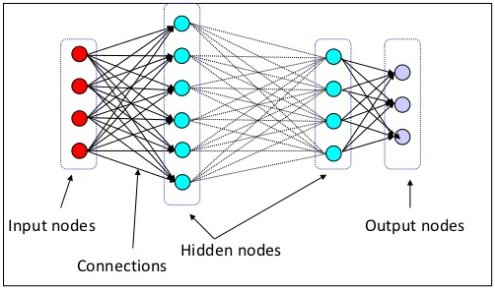
\includegraphics[ width=0.6\textwidth]{neural-networks-layers.jpg}
\end{figure}

\end{frame}

% -----------------------------------------------------------------
\begin{frame}[allowframebreaks]
\frametitle{\insertsection}

\begin{figure}
\centering
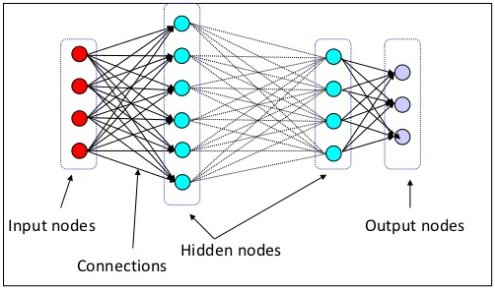
\includegraphics[ width=0.6\textwidth]{neural-networks-layers.jpg}
\end{figure}

\end{frame}

% -----------------------------------------------------------------
\begin{frame}[allowframebreaks]
\frametitle{\insertsection}

$x(t) = 0$

\end{frame}

\end{document}
